\documentclass[11pt]{article}
\usepackage[utf8]{inputenc}
\usepackage[T1]{fontenc}
\usepackage[french]{babel}
\usepackage{amsmath}
\usepackage[bookmarks={true},bookmarksopen={true}]{hyperref}
\usepackage{graphicx}
\usepackage[a4paper]{geometry}
\usepackage{listings}
\usepackage{amssymb}
\usepackage{amsmath,amsfonts}
	\lstset{frame=tb,
		language=Java,
 		aboveskip=3mm,
  		belowskip=3mm,
  		showstringspaces=false,
  		columns=flexible,
  		basicstyle={\small\ttfamily},
  		numbers=none,
 		numberstyle=\tiny\color{gray},
  		keywordstyle=\color{blue},
  		commentstyle=\color{dkgreen},
  		stringstyle=\color{mauve},
  		breaklines=true,
  		breakatwhitespace=true
  		tabsize=3
	}
\pagestyle{plain}
\setlength{\parindent}{5mm}
\usepackage{amsmath}
\usepackage{color}
\definecolor{dkgreen}{rgb}{0,0.6,0}
\definecolor{gray}{rgb}{0.5,0.5,0.5}
\definecolor{mauve}{rgb}{0.58,0,0.82}



\title{\textbf{Projet LSINF1121 -  Algorithmique et structures de données\\ - \\ Rapport intermédiaire Mission 6} \\ {\large Groupe 26}}
\author{Laurian \bsc{Detiffe} \\(6380-12-00)\and Sundeep \bsc{Dhillon} \\(6401-11-00)\and Alexis \bsc{Macq} \\ (5910-12-00) \and Xavier \bsc{Pérignon} \\ (8025-11-00)\and Thibaut \bsc{Piquard}\\(4634-13-00)\and Thomas \bsc{Wyckmans} \\ (3601-12-00)}
\date{date}
\date{\vspace*{25mm}

\includegraphics[scale=0.75]{logo.jpg}\\
		\vspace*{30mm}
		\begin{center}
		Année académique 2015-2016 \\	
		\end{center}}

\begin{document}
\thispagestyle{empty}

\maketitle
\thispagestyle{empty}
%\tableofcontents
%\setcounter{tocdepth}{3}
%\setcounter{page}{1}
%\newpage

\section*{Questions et réponses}
\begin{enumerate}

\item

\item  

\item 

\item 

\item 

\item 

\item Afin de compléter le MST partiel et retrouver un MST complet dans le graphe G, je vais appliquer l’algorithme de Kruskal. Cet algorithme est simple, il récupère tous les Lien (Edge) triés de manière croissante (plus petit poids au plus grand) et va ajouter au fur et à mesure tous ceux qui ne forme pas de cycle :
\\
\begin {verbatim}
Public static void RecoverMST(EdgeWeightedGraph G, Queue<Edge>, UF uf)
{
	MinPQ<Edge> pq = new MinPQ<Edge>(G.edges());
	while (!pq.isEmpty() && mst.size() < G.V()-1)
	{
		Edge e = pq.delMin();   		 //Get min weight edge on pq
		int v = e.either(), w = e.other(v); 	//and its vertices.
		If (uf.connected(v,w))  {continue;}	//ignore ineligible edges.
		uf.union(v,w); 				//merge components 
		mst.enqueue(e);				//Add edge to mst
	}
}
\end {verbatism}

Cet algorithme se base sur une règle fondamentale du MST, il nepeut y avoir de cycle à l’intérieur d’un MST. Grâce à « union-find », on peut savoir si deux somments sont déjà connectés ou non, et s’il faut donc traiter cet Edge (l’ajouter au MST).
\\
Il est aussi possible de régénérer l’union-find depuis le MST existant, simplement en parcourant celui-ci et en liant chacun des différents sommets dans chacune des liants de ce MST partiel.
La complexité temporelle de cette méthode est de O(Elog(E)).

\item On peut élargir ce problème à un problème de MST plus vaste, c’est-à-dire : comment mettre à jour votre MST après un Edge quelconque  ait été mis à jour dans votre Graphe ? \\
Il y a plusieurs cas possible : \\

	\begin{enumerate}
	
	\item L’edge mis à jour est dans votre MST et sa valeur décroît : il n’y a strictement rien à faire.
	\item L’edge mis à jour n’appartient pas au MST et sa valeur décroît : il faut ajouter l’Edge dans le MST, ce qui créera un 		cycle au sein du MST. Il suffit ensuite de parcourir le MST depuis un des deux Vertice de cet Edge (via BFS ou DFS) et 			retirer dans ce cycle l’Edge au poids le plus haut (Complexité O(N)).
	\item L’Edge mis à jour est dans votre MST et sa valeur croît : il faut retirer  l’Edge de cet MST, ce qui créera deux 			éléments connectés qui doivent être raccordés. On peut facilement calculer ces deux composants via DFS ou BFS (Complexité O		(N)), il faut ensuite parcourir les Edge restants par ordre croissant et ajouter le premier Edge qui relie les deux 			éléments connectés.
	\item L’Edge mis à jour ne fait pas partie du MST et sa valeur croît : Le MST actuel est toujours un MST.
	
	\end{enumerate}
\\
Maintenant, ces diffétents cas ne couvrent pas spécifiquement notre probléme tel que je le comprends, c’est-à-dire, inclure quoi qu’il arrive l4Edge e même si celui-ci ne devrait pas se trouver dans le MST. Pour arriver à résoudre ce problème, il suffit de tweaker un petit peu le cas 2. Au moment du retrait du poids le plus haut, si celui-ci est l’Edge e, alors on retirera le second plus haut.


\item 

\item Soit le graphe suivant :\\

\begin{figure}[h!]
    \center
    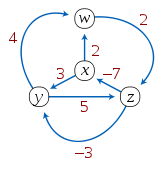
\includegraphics[width=5cm]{graph.png}
    \caption{Graphe contenant un cycle de longueur impaire (w-z-x)}
\end{figure}\\

En empruntant le cycle w-z-x une infinité de fois, on sait montrer que 
la distance minimale entre y et w est $ -\infty $ 
or en appliquant l'algorithme de Dijkstra, 
on ne peut relaxé qu'une fois chaque noeud ce qui implique qu'on ne peut parcourir
le cycle w-z-x de longueur négative qu'une et une seule fois et l'algorithme 
de Dijkstra ne pourra donc pas nous permettre d'obtenir la solution optimale,
 à savoir $ -\infty $. Il gardera toutefois la même complexité puisqu'en appliquant 
 l'algorithme de Dijkstra, on ne peut relaxé qu'une seule fois chaque noeud.\\

(Alexis)\\

\item Soit $G$ un graphe avec des poids potentiellement négatif mais il n’y a pas de
cycle négatif. Je cherche le chemin le plus court entre un noeud $u$ et un noeuds $v$.
J’ai à ma disposition une implémentation de Dijkstra qui ne permet pas de gérer
les poids négatifs. Il me suffit dès lors d’augmenter tous les poids d’une même
quantité correspondant a la valeur absolue du plus petit poids et d’appliquer
Dijkstra sur ce graphe. Cette méthode est-elle valable ? Si non, montrez un contre
exemple. (Xavier)\\

Non, c'est méthode n'est pas valable. Par exemple, considérons le graphe où il existe deux chemins de A vers B, l'un traversant un seul arc de longueur 2, et l'autre traversant des arcs de longueur 1, 1 et -2. Le deuxième chemin est plus court, mais si on augmente de 2 tous les poids des arcs (valeur absolue du plus petit poids), le premier chemin a maintenant une longueur de 4, et le second a une longueur de 6, inversant le chemin le plus courts.
\begin{center}
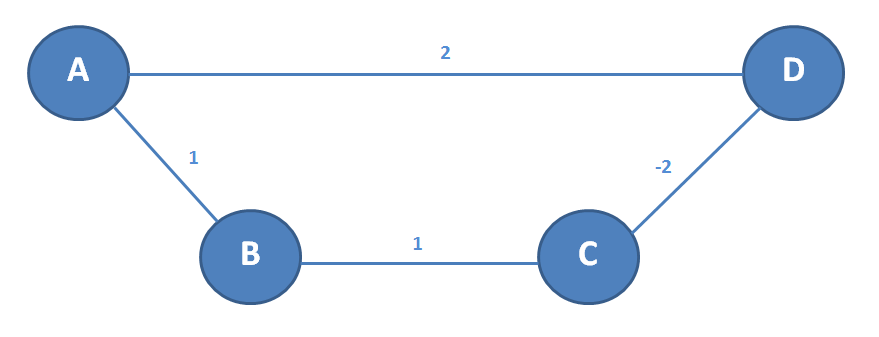
\includegraphics[scale=0.5]{dijk.PNG} 
\end{center}
Cette méthode ne fonctionnera que si tous les chemins possibles entre les deux noeuds utilisent le même nombre d'arcs.\\

\item Soit $G$ un graphe avec des poids positifs. Je cherche le chemin le plus long entre
un noeud $u$ et un noeuds $v$. J’ai à ma disposition l’implémentation de Bellman-
Ford (qui supporte les poids négatifs). Il me suffit dès lors de calculer le plus
court chemin sur le même graphe avec l’opposé des poids. Est-ce que cette méthode
est valable ? Si non pouvez-vous proposer une méthode pour le calcul de
plus long chemin ? Votre méthode s’applique-t-elle à tous les graphes ? Si non
quels-types particuliers de graphes peut-elle gérer ? (Xavier)\\

Cette méthode est valable pour certains graphes. Le principe le plus important pour l'utilisation de cette méthode est qu'il n'y ait pas de cycle dans le graphe, dans laquelle les arcs ont une somme négative. Dans ce cas, une boucle infinie serait générée et aucun plus long chemin ne serait trouvé.

\end{enumerate}
\end{document}
